%%%%%%%%%%%%%%%%%%%%%%%%%%%%%%%%%%%%%%%%%%%%%%%%%%%%%%%%%%%%%%%%%%%%%%%%
%                                                                      %
%     File: Thesis_Background.tex                                      %
%     Tex Master: Thesis.tex                                           %
%                                                                      %
%     Author: Andre C. Marta                                           %
%     Last modified :  2 Jul 2015                                      %
%                                                                      %
%%%%%%%%%%%%%%%%%%%%%%%%%%%%%%%%%%%%%%%%%%%%%%%%%%%%%%%%%%%%%%%%%%%%%%%%

\chapter{State of the Art}
\label{related_work}

In this chapter we analyze the existing work related to V2X communication. In order to have a high level understanding of how V2X communications work, we
start by specifying two vehicular PKI solutions. The first is named \textit{A Generic Public Key Infrastructure for Securing Car-to-X Communication} and has been proposed by the corresponding stakeholders in Europe \cite{generic_eu} \cite{etsi_formats} \cite{wow} (Section \ref{etsi_design}). The second is named \textit{Security Credential Management System} (SCMS) and is the American counterpart proposed in \cite{scms} (Section \ref{us_pki}). For each solution, we analyze the corresponding PKI architecture and its most relevant operational aspects such as enrollment of vehicles, revocation of certificates, and others. In Section \ref{standards}, we provide an overview the existing standards behind the European solution, which will be the basis of our work, and present a lower level and more detailed notion of the V2X communication functioning. Lastly in Section \ref{simulators}, we introduce the existing V2X communication simulators and study how they can be used to evaluate our vehicular PKI solution. 


%%%%%%%%%%%%%%%%%%%%%%%%%%%%%%%%%%%%%%%%%%%%%%%%%%%%%%%%%%%%%%%%%%%%%%%%
\section{Overview of the European Vehicular PKI Solution}
\label{etsi_design}
The European vehicular PKI solution is a generic concept so it allows some flexibility in its implementation. Our proposed PKI will primarily be based on the European solution. Specifically we aim to readjust such solution so it can be integrated in Multicert's PKI. 


%%%%%%%%%%%%%%%%%%%%%%%%%%%%%%%%%%%%%%%%%%%%%%%%%%%%%%%%%%%%%%%%%%%%%%%%
\subsection{European Vehicular PKI Architecture}
\label{section:european_pki}

The European PKI uses long-term certificates named enrollment certificates and short-term certificates known as pseudonym certificates or \textit{Authorization Tickets} (ATs). Enrollment certificates are tied to the vehicle's identity to authenticate the vehicle within the PKI back-end. Authorization tickets have the identifying information removed and are used in V2X communications for privacy reasons. The European PKI considers an hierarchical structure as we can see in Figure \ref{fig:ETSI_PKI}. Such architecture is composed of a \textit{Root Certification Authority} (RCA), an \textit{Enrollment Authority} (EA), and an \textit{Authorization Authority} (AA). For a given trust domain the RCA certificate is the root of trust for all certificates in that hierarchy, this means that a vehicle will only trust an incoming message if the certification chain starting on the received authorization ticket to the root CA certificate is valid. The RCA is responsible for issuing certificates for enrollment authorities and authorization authorities. If there are multiple RCAs, trust between them can be established by using cross certification. No other cross certification between CAs is allowed. The EA has the responsibility of validating that a vehicle can be trusted and only if so, issuing an enrollment certificate for that vehicle as a proof of its identity. Finally, the AA exists to allow vehicles to apply for specific services and permissions on the road. These privileges are denoted by means of authorization tickets (pseudonyms), which are issued by the AA for the applying ITS-S.



\begin{figure}
	\centering
	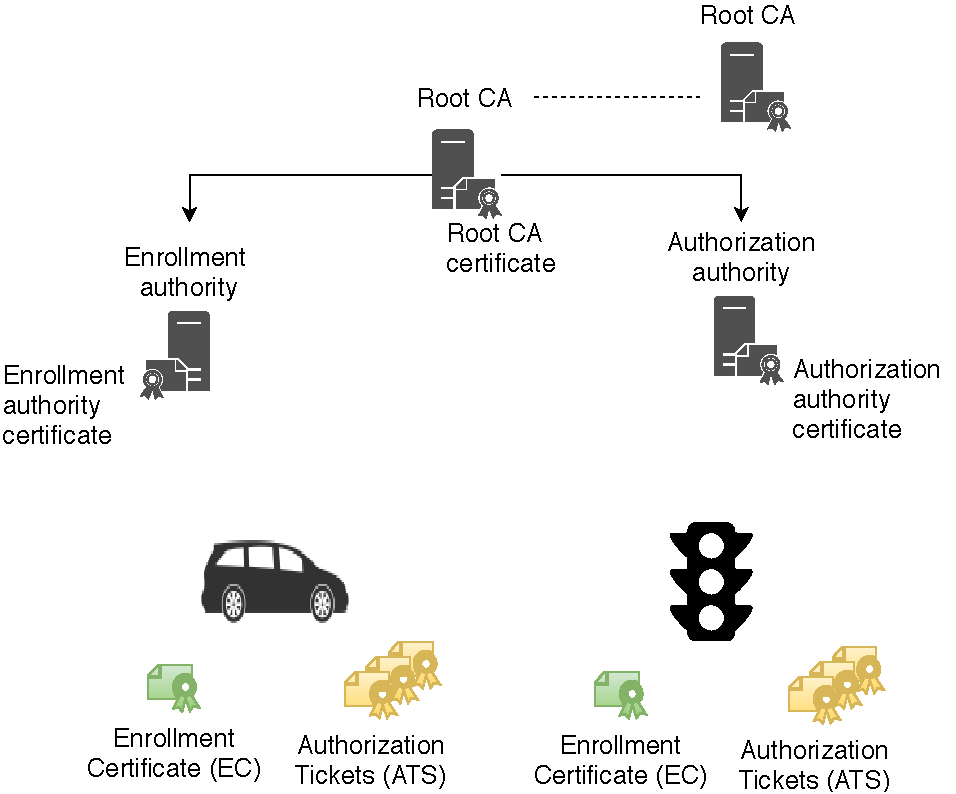
\includegraphics[width=0.8\textwidth]{Figures/ETSI_PKI.pdf}
	\caption{\label{fig:ETSI_PKI}European vehicular PKI architecture.}
\end{figure}

%%%%%%%%%%%%%%%%%%%%%%%%%%%%%%%%%%%%%%%%%%%%%%%%%%%%%%%%%%%%%%%%%%%%%%%%
\subsection{ITS-S Security Life Cycle}
\label{section:life-cycle}

The ITS-S security life cycle is relevant for our solution because through its analysis we are able to understand which stages every vehicle undergoes during its lifetime. Each stage involves a change in the vehicle's state against the PKI. The analysis of such stages allows us to understand when and what information needs to be initialized in the vehicles and transferred between vehicles and the PKI. Specifically, which variables need to be initialized in the vehicles’ OBU at bootstrap, what needs to be done regarding the vehicle enrollment and authorization, and how can we update PKI management information throughout the life cycle of the vehicles.
ETSI TS 102 941 \cite{etsi_privacy} standards specify the ITS-S' security life cycle comprising four stages: the manufacture, enrollment, authorization and maintenance. The first stage of an ITS-S' life cycle is the manufacture, it is at this stage that all the information needed for the enrollment is initialized within the station itself (OBU) and within the EA. The next stage is the enrollment where the ITS-S requests its enrollment certificate from the EA. Having received the enrollment certificate, the ITS-S can now request authorization tickets from the AA. The request for authorization tickets represents the authorization stage. 

When a vehicle is manufactured the OBU and EA need to be initialized. Within the vehicle's OBU, it is necessary to provide information regarding the vehicle's identity and information to allow the vehicle to interact with the PKI. Regarding the identifying information, a unique identifier and a public\slash private key pair to be used for cryptography are created. Optionally, a canonical certificate can be installed which associates the canonical identifier with the public key of the vehicle. In this case, the certificate chain back the root authority needs also to be installed. To allow a vehicle to connect to the PKI, it is necessary to install the network address and public key certificate of the EA and AA that will issue certificates for that vehicle. In addition, the set of known and trusted EA certificates is installed to allow the vehicle to initiate the enrollment process. To grant that such vehicle is able to verify the authenticity of incoming V2X messages, the set of known and trusted AA certificates must also be provided. In order to support vehicle enrollment, within the EA it is necessary to provide information that identifies the manufactured vehicle: a unique vehicle identifier, the location profile information for the vehicle, and the public key that belongs to the vehicle's key pair. In the next sections we study how the European Vehicular PKI operates regarding the provisioning of certificates, their revocation, and how the messages are signed and verified by the user vehicles. Our vehicular PKI must support such operational aspects.

\subsection{Enrollment Process}

Before an ITS-S is able to participate in the V2X communication it must be registered within the PKI. The enrollment request message should be sent from the ITS-S to the Enrollment Authority, to protect the users' privacy the request must be encrypted. According to ETSI TS 102 941 \cite{etsi_privacy} this message should contain the following fields:
\begin{itemize}
	\item{ Message signer information, i.e. the canonical certificate or the public key provided to the ITS-S at bootstrap to globally identify it.}
	\item{ certificate request, i.e. the information to be presented in the enrollment certificate. For example, the ITS-S' public key, start time, end time and other certificate specific data.}
	\item{ The digital signature of the message sender (requesting ITS-S) calculated over all message fields.}
\end{itemize}
After the ITS-S enrollment request the target EA must reply with a successful or failed response message, to protect user privacy the response should also be encrypted. The successful ITS-S enrollment response should contain the enrollment certificate and the chain of certificates back to the originating enrollment CA. In the failed ITS-S enrollment, the response contains the error code i.e. the reason for the unsuccessful enrollment response. 


\subsection{Authorization Ticket Provisioning}
\label{section:at_usage}

Pseudonym certificates are short-lived certificates which express the permissions that a specific enrolled vehicle has on the road while hiding its identity. Consequently, they are refereed as \textit{Authorization Tickets} (ATs) by ETSI. To avoid long-term tracking, a vehicle rotates authentication tickets from its local pool to authenticate V2X messages. However, it needs to request new ATs from the authorization authority once there are few valid ATs stored locally. The update can be done over-the-air or at an authorized dealership (during vehicle maintenance), i.e. roadside-units and workshops can act as a proxy for certificate requests. Because our solution will also use ATs, important decisions must be done regarding the frequency that ATs are provisioned to the enrolled vehicles and how such vehicles rotate certificates from their pool. There is the need to adopt a model that specifies the authorization ticket provisioning. The model used in Europe is defined in CAR 2 CAR Communication Consortium (C2C-CC) \cite{generic_eu}. In this model the required frequency of updates, the delivered level of privacy and security can be expressed by three determining parameters:

\begin{itemize}
	\item{ \textbf{Certificates valid simultaneously:} It can be defined that the requester can use several ATs with the same start and expiry date.} 
	\item{ \textbf{Authorization ticket validity time period:} Is defined by the time between start and expiry timestamps of the ATs.}
	\item{ \textbf{Overall covered time-span:} The time that is covered by the batch of authorization tickets.}
\end{itemize}

A vehicle receives a ``super-batch'' that contains a set of ATs, the duration of the ``super-batch'' is the \textit{overall covered time-span} and is in the order of years. The ``super-batch'' is composed of ``sub-batches'' which contain a sub-set of certificates (e.g., 20) valid for the same time period (e.g., a week). During that week the vehicle uses and reuses the 20 valid certificates. The certificate usage pattern can vary from device to device, e.g. a device could use a certificate for 5 minutes after start-up, then switch to another certificate, and use that either for 5 minutes, or until the end of the journey. Figure \ref{fig:AT_P} illustrates this method. 

\begin{figure}
	\centering
	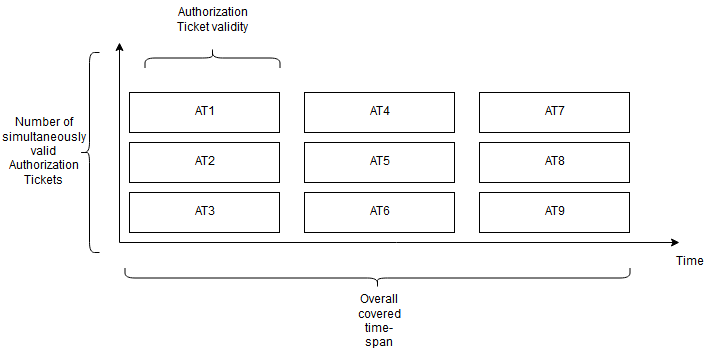
\includegraphics[width=0.8\textwidth]{Figures/AT_P.png}
	\caption{\label{fig:AT_P}Authorization Ticket provisioning model.}
\end{figure}

\subsection{Authorization Ticket Request Process} \label{auth_process}
In this section we study the sequence of messages used by vehicles to request valid ATs in Europe. The solution that we propose will assume such protocol for the simulated vehicles' requests for ATs.
At a high level, a vehicle uses its enrollment certificate to prove its enrollment to the AA, only then the AA can issue the ATs.
The ETSI TS 102 941 \cite{etsi_privacy} standard specifies in detail the message format for the AT request and response. In regards to the process \cite{generic_eu}, the vehicle sends a request to a predefined AA. The request includes the vehicle's enrollment certificate, the certificate of the corresponding Enrollment Authority, and the to be certified public key. To protect user's privacy the enrollment certificate may be encrypted with the public key of the corresponding EA. In this case the AA is not able to create a link between the authorization tickets and the enrollment certificate of a specific vehicle. Consequently, when an AA receives such requests it cannot verify the enrollment of the requesting vehicle. In order to do so, the AA sends a request with the (encrypted) vehicle's enrollment certificate and the calculated AT overall covered time-span (e.g. 1 year) to the correct EA (identified by the EA certificate present in the original request). The EA maintains a database that stores a timestamp marking the deadline which the vehicle will still have valid ATs (calculated using the overall covered time-span of the request). Only if the vehicle's enrollment certificate is valid and no ATs are issued for the time which the vehicle still has valid ATs the AA will get a positive response from the EA validating the enrollment of the vehicle. Upon receiving such response, the AA has the responsibility of issuing the ATs for the vehicle. This procedure prevents a vehicle from requesting ATs for the same time interval from different or the same AAs.


\subsection{Message Signing and Verification}

In this section we analyze how the secured V2X messages are signed and verified by the vehicles. Such information will allow us to correctly test the communications between vehicles in the proposed simulator. In regard to sending messages, the sender of V2X messages signs all outgoing messages with the private key of a valid AT. Afterwards, the message with the appended signature and pseudonym certificate is broadcast. When a station receives a message, the senders authenticity and message integrity is verified by decrypting the signature with the public key from the appended AT. The sender's authenticity is only accepted if verification of the received AT up to a root CA is possible. Vehicles are preloaded with the known and trusted authorization authority certificates at manufacture. However, if the Authorization Authority certificate that corresponds to the received AT is not locally stored, the message receiver cannot validate the sender's authenticity. In this case, the message receiver must create a new message requesting the missing Authorization Authority certificate and send it to the original message sender. Then, the receiver of this request must respond with the Authorization Authority certificate (more details present in Section \ref{standards}).

\subsection{Certificate Revocation}

Sometimes it may be necessary to remove bad actors from the system. This requirement influences the architecture of the PKI, namely there must be an entity responsible for detecting misbehaving actors. Once detected, a bad actor must be removed from the communication. 

In the European solution detecting and preventing misbehavior by means of a misbehavior entity is not yet supported. Revocation is done in respect to the long-term enrollment certificate of ITS-S and CA certificates. ITS stations are eventually removed from the system by rejecting new requests for ATs. In this concept the EA links the revocation information of the vehicle to its long-term enrollment certificate. If the vehicle requests new ATs then the AA forwards the request to the respective EA which checks the revocation information of the requester. In respect to the revocation of any CA certificate a distributed \textit{Certificate Revocation List} (CRL) is used. In this scheme, the CA certificates that are compromised are revoked manually by the PKI administration; the certificate identifier is posted in the CRL and signed by the root CA; finally, the CRL is distributed inside the PKI backbone and connected ITS stations. The CRL for EA and AA certificates is defined in ETSI TS 102 941 \cite{etsi_privacy} standard.

\section{Overview of the American Vehicular PKI Solution} \label{us_pki}
In this section we provide an overview of the Security Credential Management System as a matter of reference. Although this theses follows the European PKI solution, it is relevant to reference the American vehicular PKI in order to understand the main differences and similarities between solutions.
In comparison to the architecture of the European vehicular PKI the American counterpart is noticeably more complex. However, it shares some similarities with the European vehicular PKI. The main differences include an increased focus on privacy against attacks from SCMS insiders, the handling of certificate revocation, and the method for provisioning certificates based on the butterfly key expansion algorithm. 

\subsection{American Vehicular PKI Architecture}
\bigbreak
SCMS considers an hierarchical structure as we can see in Figure \ref{fig:SCMS_PKI}. Comparing with the European vehicular PKI architecture, there are some components with a similar function and others that introduce new functionality. In regard to the similar components, SCMS assumes a \textit{Root CA}, an \textit{Enrollment CA}, and a \textit{Pseudonym CA} (PCA) which corresponds to the authorization authority in the European architecture. As to the remaining components, their functionality is as follows:

\begin{itemize}
	\item \textbf{Device Configuration Manager (DCM):} Provides authenticated information about changes in the configuration of SCMS's components, for example an authority changing its certificate. It is also used to inform an enrollment CA that a device is eligible to receive enrollment certificates.
	\item \textbf{Registration Authority (RA):} Validates, processes, and forwards requests for pseudonym certificates to a pseudonym CA.
	\item \textbf{CRL Store (CRLS):} Stores and distributes CRLs. CRLs are signed by the CRL Generator.
	\item \textbf{CRL Broadcast (CRLB):} Broadcasts the current CRL, may be done through road side units or satellite radio system, etc.
	\item \textbf{Linkage Authority (LA):} The main goal of this component is to improve certificate revocation. LAs generate linkage values, which are used in the certificates and support efficient revocation (more on this later). There are two LAs in the SCMS, referred to as LA1 and LA2. The splitting prevents the operator of an LA from linking certificates belonging to a particular device. 
	\item \textbf{Location Obscurer Proxy (LOP):} The main goal of this component is to improve the security against SCMS insiders. The LOP hides the location of the requesting device by changing source addresses. Additionally, when forwarding information to the Misbehavior Authority (MA), the LOP shuffles the reports to prevent the MA from determining the reporters’ routes.
	\item \textbf{Misbehavior Authority (MA):} Processes misbehavior reports to identify potential misbehavior by devices, and if necessary revokes and adds devices to the CRL. It also initiates the process of linking a pseudonym certificate to the corresponding enrollment certificates, and adding the enrollment certificate to an internal blacklist.
	\item \textbf{Request Coordination (RC):} Ensures that a device does not request more than one set of pseudonyms for a given time period. It coordinates activities between different RAs.
\end{itemize}

An early version of SCMS has already been implemented, operated and tested in the safety pilot project \cite{safty_pilot}. Safety pilot is a scaled-down evaluation of V2X that uses real vehicles and roadside infrastructure in order to understand the safety benefits of connecting vehicles. SCMS documentation can be found in \cite{scms_doc}

\begin{figure}
	\centering
	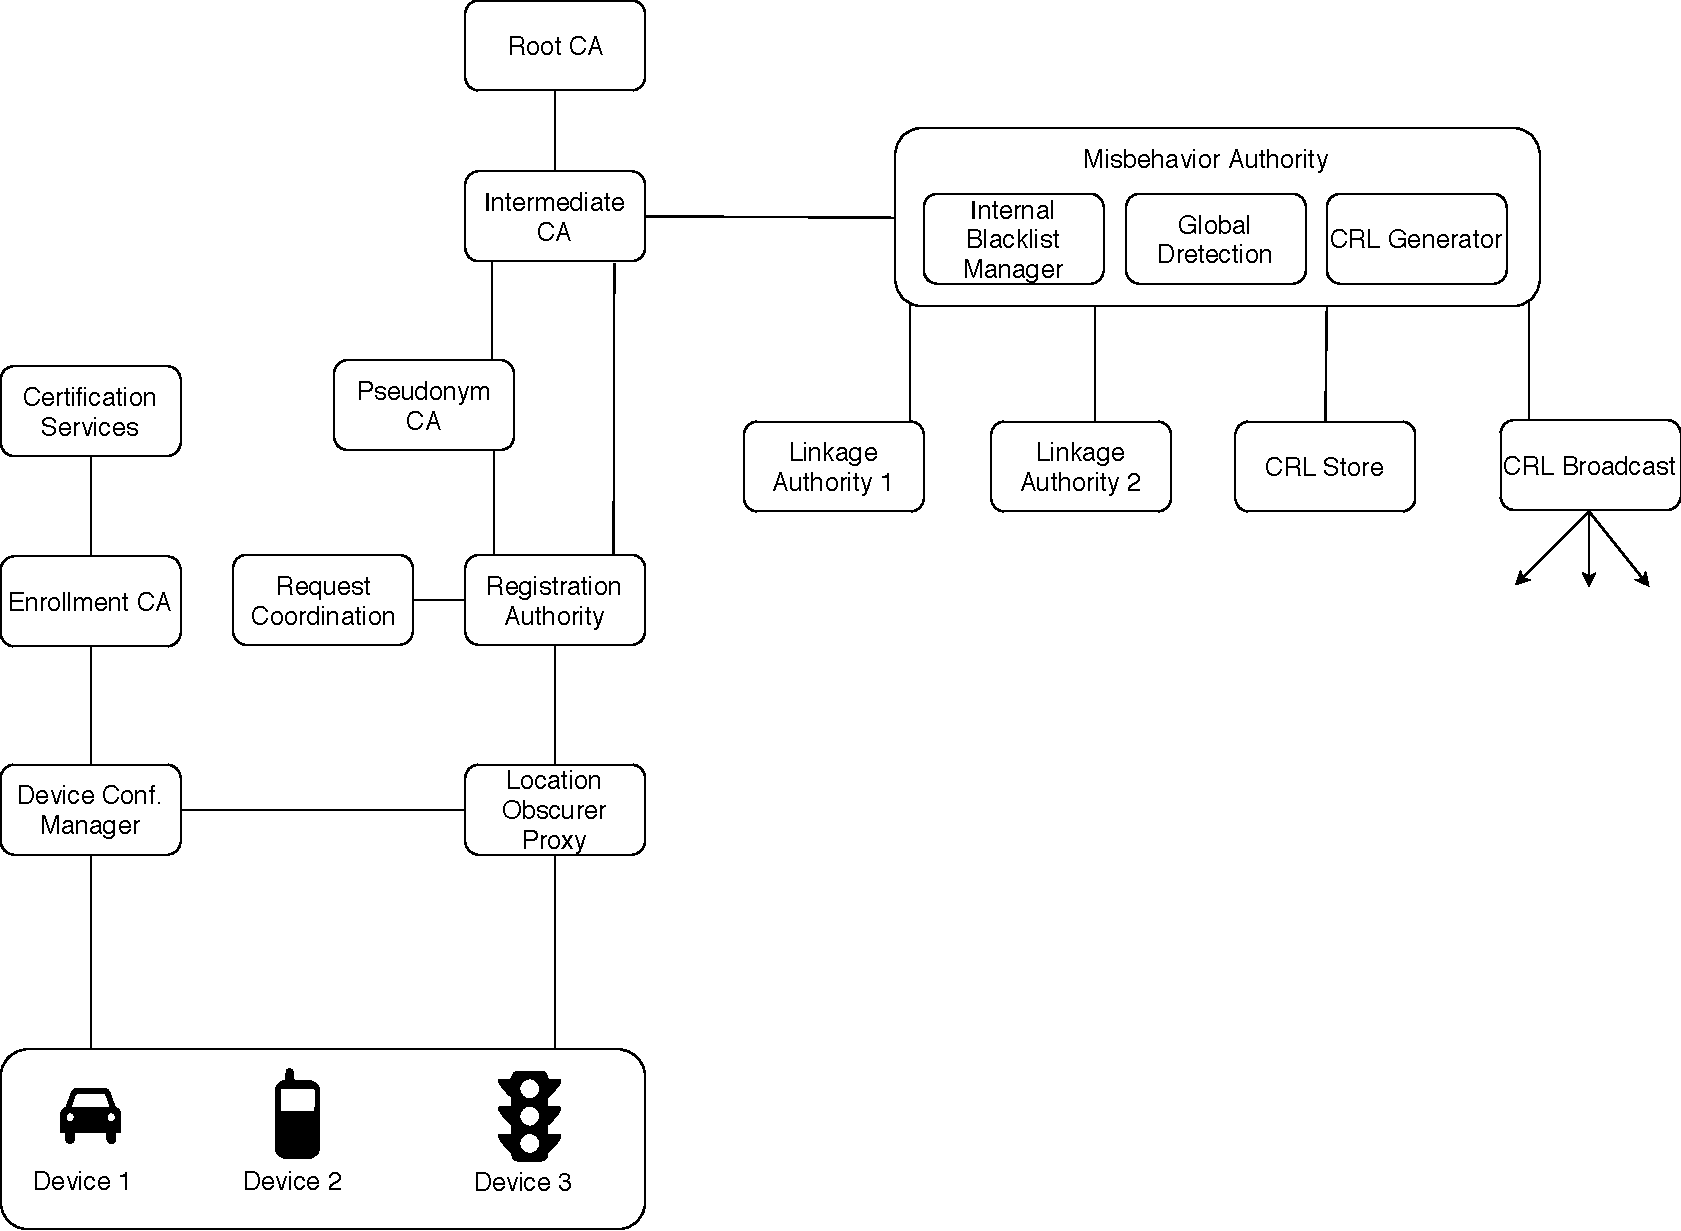
\includegraphics[width=0.8\textwidth]{Figures/SCMS_PKI.pdf}
	\caption{\label{fig:SCMS_PKI}SCMS overall system architecture.}
\end{figure}

\subsection{Pseudonym Certificate Provisioning Model}
\bigbreak
Regarding the model used for provisioning pseudonym certificates, the SCMS assumes the same model as in CAR 2 CAR Communication
Consortium \cite{generic_eu} (European solution) illustrated in Figure \ref{fig:AT_P}. The proposed parameters for this model are:
\begin{itemize}
	\item \textbf{Certificate validity time period:} 1 week.
	\item \textbf{Certificates valid simultaneously (batch size)}: 20 to 40 certificates.
	\item \textbf{Overall covered time-span (super-batch size):} 1 to 3 years.
\end{itemize}

\subsection{Pseudonym Certificate Request Process}

The request for pseudonym certificates in itself is different from the European solution. For this the
butterfly key expansion algorithm \cite{scms} is used. Butterfly keys allow a device to request an arbitrary number of certificates, each encrypted with a different encryption key and each containing a different signing key. The request contains only one seed for the verification public key, one seed for the encryption public key, and two expansion functions. Without butterfly keys, vehicles would have to send a signing key and a unique encryption key for each requested certificate. Butterfly keys reduce upload size, allowing requests to be made even in suboptimal connectivity conditions, and also reduce the computation to be done by the vehicle to calculate the keys. More information about the request process can be found in \cite{scms}.


\subsection{Misbehavior Reporting}

In contrast to the European PKI, the American PKI supports misbehavior reporting by user vehicles. This feature aims to improve the security against SCMS outsiders by reporting their malicious messages. 
Devices will send misbehavior reports to the MA via the LOP which will obscure the source and shuffle the reports from multiple reporters, this is done to prevent the MA from reconstructing the reporter’s path based on the reports. The format of a misbehavior report is not fully defined yet, but a report will potentially include reported messages in addiction to the reporter’s signature and certificate, and will be encrypted by the reporter for the MA.

\subsection{Global Misbehavior Detecting and Revocation}

The algorithms necessary for global misbehavior detection have not been developed at the time of this writing. However, the interface which allows SCMS components to retrieve linkage information is already specified.
Revocation is tightly bound to the linkage information which basically allows the MA to find whether multiple reported messages point to the same device.
The revocation process is described step-by-step in \cite{scms}. In this section we learned about the European and American vehicular PKIs and about their most relevant operational aspects. In the next section we present the standards which shape the formats of the certificates and messages used in the European vehicular PKI.

\section{Secured Message and Certificate Formats Standard}\label{standards}
One of the main concerns of V2X communication is the ITS interoperability. Standardization of the communication protocol becomes fundamental with so many vehicles from different manufacturers using the road and sharing information. To achieve this goal there are dedicated work groups within standardization organizations that address security and privacy concerns. While ETSI Automotive Intelligent Transport Systems represents the main standardization stakeholders in Europe \cite{etsi_workgroup}, IEEE 1609.2 represents the main standardization stakeholders in the U.S \cite{iee_formats}. Such standardization efforts are the basis of the security and privacy of the European and American vehicular PKI solutions respectively. A survey about recent standardization activities in Europe (ETSI) has been done by IEEE in \cite{wow}.

Regarding the secured message and certificates formats. IEEE 1609.2 \cite{iee_formats} standard defines the formats for secured V2X messages and public key certificates to be used in SCMS. In this standard the V2X message authenticity and integrity are based on the \textit{Elliptic Curve Digital Signature Algorithm} (ECDSA). The message confidentiality protection is based on AES symmetric encryption (AES-CCM mode). For the transport of symmetric keys the \textit{Elliptic Curve Integrated Encryption Scheme} (ECIES) is used. ETSI TS 103 097 standard \cite{etsi_formats} assumes the same cryptosystem as IEEE 1609.2 and presents security profiles for the messages and certificates also based on the IEEE 1609.2 standard. This means that ETSI's profiles are specific types of messages and certificates which are based on particular options available on the definitions of the base standard. For example, ETSI TS 103 097 uses the definition of possible fields that a certificate may contain (the format) present in IEEE and, based on these options, builds the specific profiles (the necessary fields) for the root CA certificates, authorization tickets, enrollment certificates, and other certificates to be used in the European solution. The same process applies with the profiles for the secured V2X messages. 

The V2X ecosystem that we propose will be primarily based on the European PKI. Consequently, it is relevant that we understand the contents of the secured V2X messages and the certificates used by it. In order to do so, we provide an overview of the ETSI TS 103 097 standard. 

\begin{figure}
	\centering
	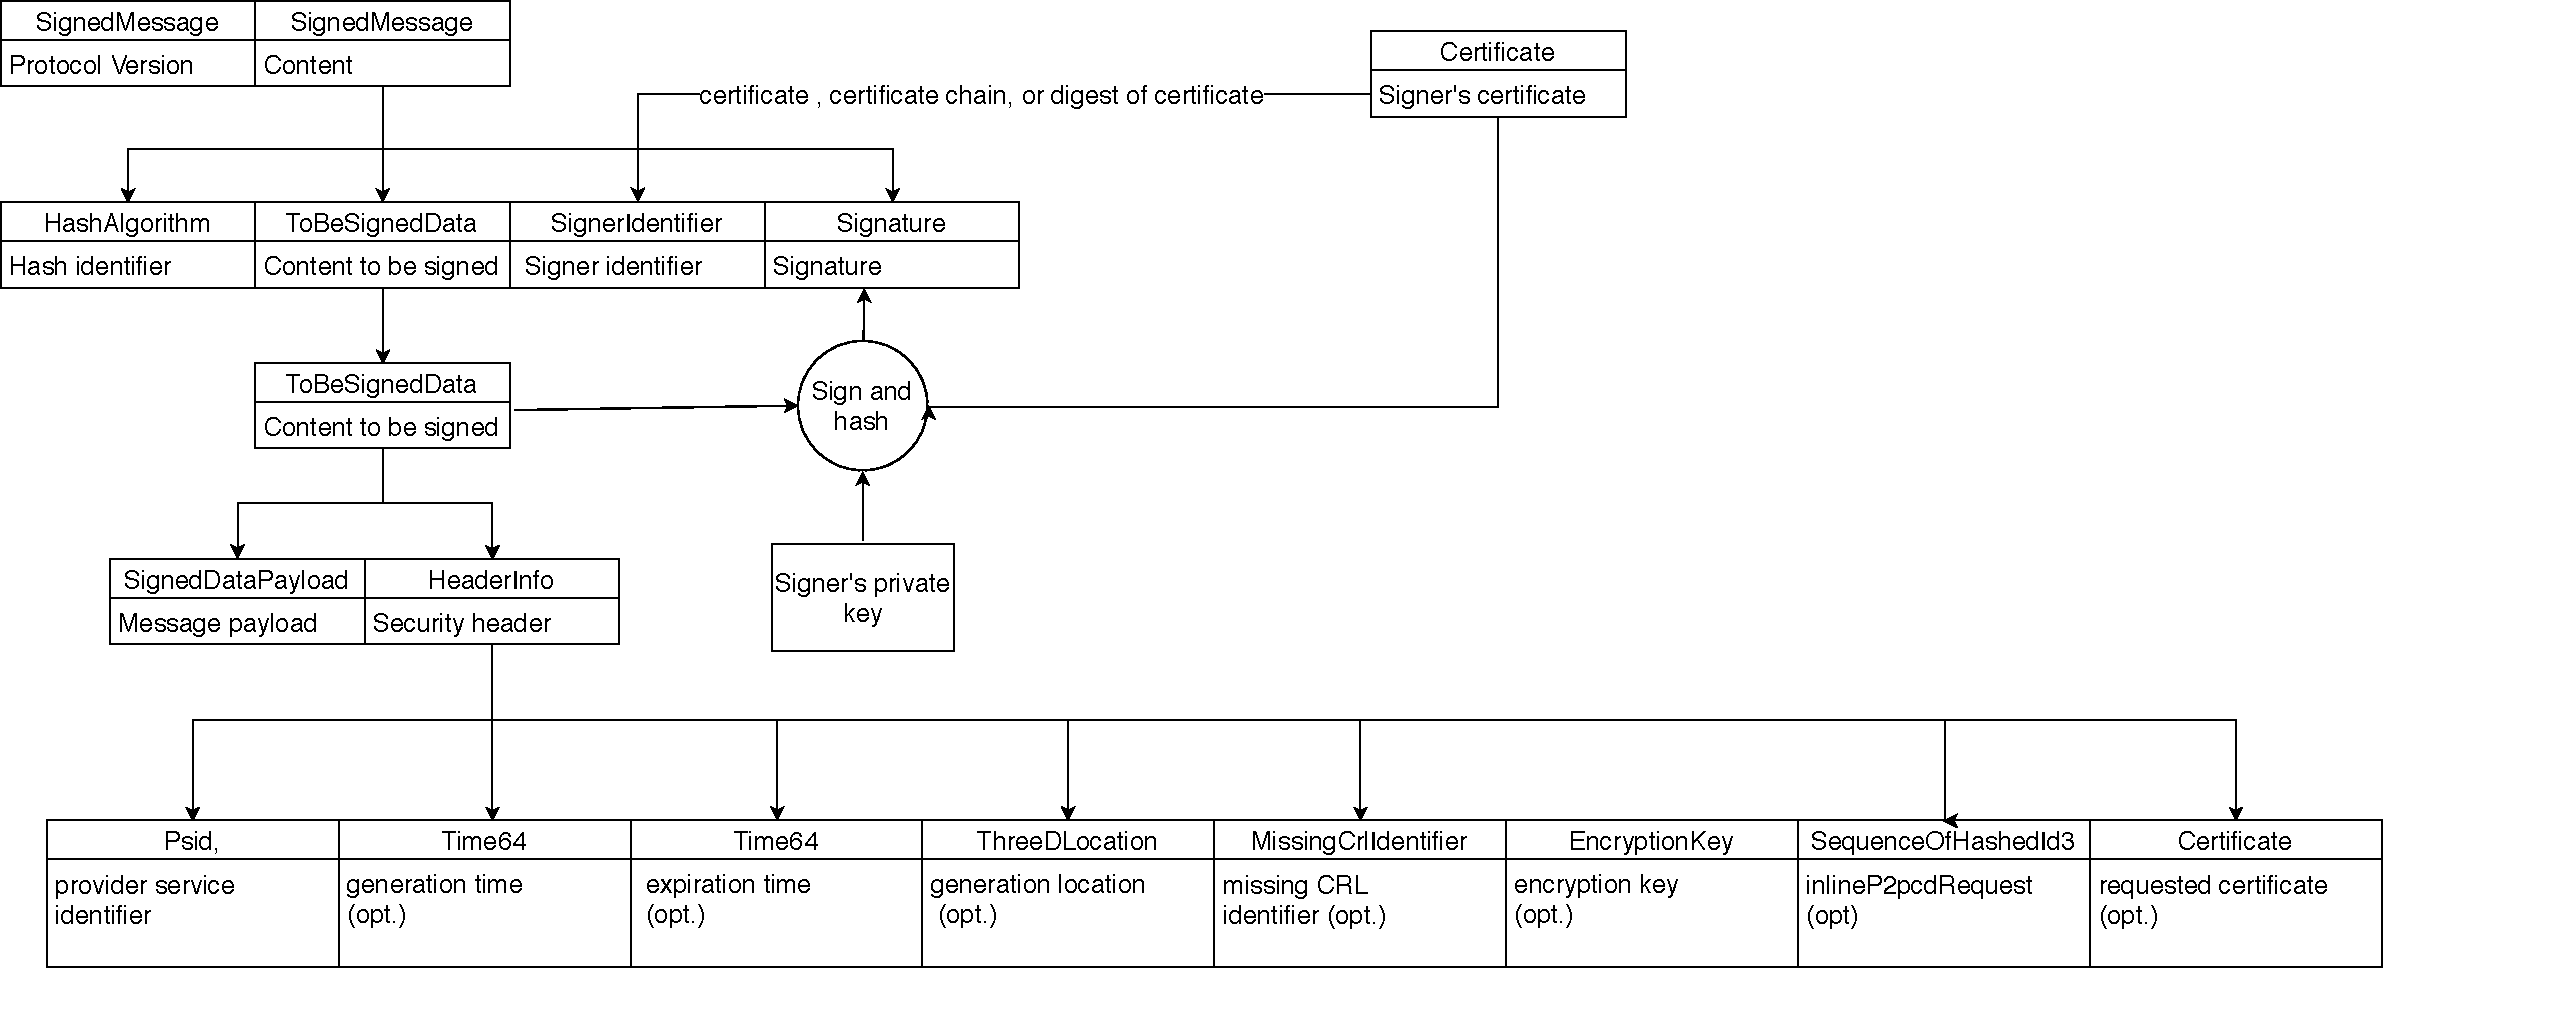
\includegraphics[width=1.1\textwidth]{Figures/message_format.pdf}
	\caption{\label{fig:signed_message}IEEE 1609.2 signed message format used by ETSI TS 103 097.}
\end{figure}

\subsection{Secured Messages Formats}
Figure \ref{fig:signed_message} depicts the format of a secured message. Generally a message can be transmitted as unsecured data, signed, encrypted, or signed and encrypted data. In the case of road security messages, the message should be signed and thereby include the hash algorithm, the content to be signed, the signer identifier, and the signature itself. Such security messages need to carry the signing certificate (authorization ticket) to reduce the processing delay at the receiver side. However, in order to reduce the network bandwidth consumption it is possible to include in the message a reference to the signing authorization ticket. For this purpose, the message signer identifier contains the certificate identifier as the 8 bytes certificate digest instead of the full certificate. 

The content to be signed includes all the message components that will be protected by the signature. Such components are the security header and the message payload. The security header includes components that are relevant for the security layer, such as the provider service identifier and some optional message validation data (generation time, expiration time, generation location, missing CRL identifier, encryption key, \textit{inlineP2pcdRequest,} and requested certificate).



A message is signed by an authorization ticket, which is turn is signed by an authorization authority certificate. Consecutively the authorization authority certificate is signed by a higher authorization authority certificate. The chain ends at a root CA certificate which issued itself. At a high level, at least one certificate in this chain must be known and trusted by the receiving station in order for it to be able to trust an incoming message.

The message receiver needs to be able to construct a chain from the message signing certificate to a known root. However, vehicles are constantly rotating authorization tickets to sign safety messages, normally exchanging only a reference to that certificate (authorization ticket hash). In addition, in many cases vehicles share the road with previously unknown vehicles for the first time. There needs a peer-to-peer (p2p) mechanism to distribute certificates on the road. This mechanism in embedded into the secured messages, specifically the receiver can use the \textit{inlineP2pcdRequest} component of a message to request unknown certificates from other senders. This functionality allows us test the correctness, performance and overhead of the distribution of unknown authorization tickets on the road.

\subsection{Secure Messages Profiles}
In the previous section we learned about the possible message components and their meaning. Here, we analyze the already standardized safety message profiles for the \textit{cooperative awareness messages} and \textit{decentralized environmental notification messages}. For each type of message, we analyze their goal, how they are sent, and how they are received by the vehicles. The proposed simulator will implement the V2X communications between simulated vehicles. As such, it assumes these two specific types of messages secured by the ATs provided by the proposed vehicular PKI.

\subsubsection{Security Profile for Cooperative Awareness Messages}
\textit{Cooperative Awareness Messages} (CAM) are messages that are exchanged between ITS-S. As the name implies, these messages are used to achieve cooperative awareness on the road. This means that road users such as vehicles (cars, trucks, trains, etc.), road-side units (traffic lights, gates, barriers, etc.) and people are aware of each other's positions, speed and other dynamic variables. To achieve this goal, it is essential that this type of messages is periodically broadcast by each road user to all its neighbors. CAMs are used to support traffic management and safety services. In the normal cases CAMs are sent multiple times per second with the component signer identifier containing the reference of the signing authorization ticket (8 byte certificate digest). However, in order to distribute the currently used AT, every second a CAM is sent with the signer identifier containing the full certificate. If a vehicle receives a CAM signed by a previously unknown AT, it should include the currently used AT immediately in its next CAM, instead of including just the digest. In this case, the timer for the next inclusion of the full certificate should be restarted to one second. 

Besides distributing the currently used AT a vehicle also needs to request the unknown certificate present on the revived CAM for message verification purposes. Specifically, if a vehicle receives a CAM with the signer identifier containing an unknown certificate digest, then it will include that digest in the component \textit{inlineP2pcdRequest} of its next CAM to broadcast the request for the full certificate. 
It is also possible for a vehicle to receive a CAM containing the full signing authorization ticket but this certificate is signed by an unknown authorization authority certificate. In this case the vehicle should include in the \textit{inlineP2pcdRequest} of its next CAM the digest of the unknown authorization authority certificate which is present on the AT itself (see more in Section Certificate formats).

If a vehicle receives a CAM containing a request for an unknown certificate i.e. with the component \textit{inlineP2pcdRequest} on the security header, then the vehicle searches the list of certificate digests existing in that component. If the digest of the currently used authorization ticket is found in that list, then it includes the full certificate in the component signer identifier of its next CAM instead of the digest. In the case that a vehicle finds a digest referencing a valid authorization authority certificate in that list, it should include such certificate in the component requested certificate of its next CAM to broadcast the response. It is possible that multiple neighbor vehicles have stored the requested AA certificate, in order to prevent unnecessary broadcast responses, a vehicle only includes the AA certificate in its next CAM if before the generation of this message no other CAM was revived containing the AA certificate in the component requested certificate.


\subsubsection{Security Profile for Decentralized Environmental Notification Messages} 
\textit{Decentralized Environmental Notification Messages} (DENM) are messages designed to provide asynchronous warning notifications to vehicles. DENMs are event triggered and are broadcast to notify the users of a hazardous event. For example, an emergency vehicle approaching or an accident on the road. These messages have to be broadcast to all users affected by the event, sometimes multiple hops are needed to achieve this.

In order to reduce the verification delay at the receiver side CAMs are always sent with the full signing authorization ticket in the signer identifier. Because it is important for vehicles to know were the event occurred, these messages will always include in the header the generation location.

\subsection{Certificate Formats}\label{cert_formats}
In the previous sections we have seen the secured message formats and profiles, which are relevant for V2X communications. In this section we introduce the existing certificate formats, which are relevant to secure such messages. Our goal is to encode such formats in a Java package and then integrate it into mPKI.


The certificate formats include profiles for the root CA, enrollment authority, authorization authority and end-entities certificates (authorization tickets and enrollment certificates).
Generally a certificate is composed of the issuer identifier, certificate identifier, application permissions, permitted geographic location, start of the validity time, expiration time, public key and the signature. In order to construct the certification chain, each non-root certificate carries the issuer identifier which is a reference (8 byte digest) that points to the certificate that belongs to the issuer CA. For example, authorization tickets carry the digest of their corresponding authorization authority certificate. The certificate identifier is a unique name that identifies the certificate's host (i.e. name of a certification authority in the case of CA certificates). The application permissions contain one or more pairs of \textit{Provider Service Identifier} (PSID) and \textit{Service Specific Permissions } (SSP). While PSID indicates a specific service, message or application the SSP indicates the permissions within that service. For example, there may be an SSP value associated with PSID of a CAM that indicates that the vehicle is privileged to send such message for a specific vehicle role (e.g emergency vehicle) or for a specific roadside unit (e.g traffic lights).

\subsection{Signed Message Validity Checks}

Before a vehicle is able to trust an incoming message it must check the message's validity. This is done by verifying that no certificate in the certification chain is revoked and the signing certificate chains to an already trusted CA certificate.
Also, the signature present in the message can be verified using the public key expressed in the certificate. The message payload must be consistent with the permissions expressed in the certificate (by the PSID/SSP pairs). Finally, the message must not be expired, i.e. the message validity is within the certificate's validity period and the message was generated within the permitted geographic location of the signing certificate. Figure \ref{fig:relation} depicts the consistency between a signed message and the signing authorization ticket.

\begin{figure}
	\centering
	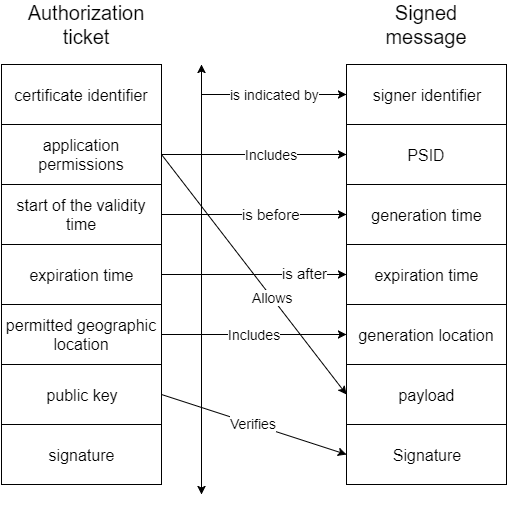
\includegraphics[width=0.5\textwidth]{Figures/relation.png}
	\caption{\label{fig:relation}Relation between a signed message and the signing certificate.}
\end{figure}


\section{Overview of the ITS Simulators}\label{simulators}
Implementing V2X communication is expensive and may prove to be dangerous to test using real vehicles. Furthermore, to properly measure the benefits of V2X communication we need to evaluate it at a large scale, for example hundreds of ITS-S. Before we can conduct a field test, a simulation framework which is able to test the communications between vehicles and infrastructure of whole cities is needed. This implies simulation at three different domains: traffic simulation to generate the road networks and traffic demand; network simulation to allow vehicle connectivity by wireless technology (e.g. IEEE 802.11p
DSRC, and IEEE 1609.4 WAVE) \cite{network_vehicle} \cite{network_vehicle2}; and ITS application simulation to trigger the communication. 
In this section we list some of the most known ITS simulators. A survey on the most known simulation tools and techniques for vehicular communications and applications can be found in \cite{sims}.

\subsection{Vehicle Mobility and Networking Simulators} 
Vehicle mobility simulators are specialized in generating the road networks and traffic demand. At this level of simulation it is important to support: a realistic representation of traffic flow that may range from a single road junction to a whole city; the support for adding new functionality and integration with other simulation tools (e.g. an interface that allows retrieving traffic simulation data and control the simulation using external functions). In this category of simulators there are two promising candidates: SUMO \cite{SUMO} and VISSIM \cite{vissim}. Network simulators have the responsibility of representing the network protocols that transmit ITS information through the VANET, to a back-end or Internet service. In this category of simulators there are three promising candidates: ns-3 \cite{ns3}, OMNeT++ \cite{omnet} and JiST\slash SWANS \cite{jist}.


\subsection{Integrated ITS Simulators}
Integrated ITS Simulators are frameworks that couple different domain simulators in order to create a functional V2X environment. At this level of simulators it is important to support a bidirectionally-coupled simulation \cite{bidirectional} of road traffic and network traffic (the mobility of vehicles affects communication and vice-versa). In this category of simulators there are three promising candidates: Veins \cite{bidirectional}, iTETRIS \cite{iTetris}, and VSimRTI \cite{vsimrti}.


\section{Discussion}
In this section we provide a brief overview of the vehicular PKI solutions presented and analyze their advantages and disadvantages.
We have seen that in Europe exists \textit{A Generic Public Key Infrastructure for Securing Car-to-X Communication} \cite{generic_eu} and in America exists the \textit{Security Credential Management System} \cite{scms}. In regard to the European PKI, the first disadvantage comes in the vehicle's request for authorization tickets. This solution assumes that every vehicle has to calculate a list of keypairs containing one signing and verification key for each of the requested authorization tickets. Since vehicles typically request a bundle of certificates to be used in a timespan of years, the generation of keys results in an increased computing overhead within the OBU whenever a vehicle needs to request new Authorization tickets. In addition, this process also increases the size of the request, which has to contain all the verification keys. The second disadvantage comes in the revocation of certificates. The European PKI does not consider distribution of CRLs containing authorization tickets within the vehicular network. As a result, this solution allows a window of vulnerability where malicious vehicles have their enrollment certificate revoked but still have a pool of valid authorization tickets, which allows them to send authenticated message for the duration of that pool. Although this system has these disadvantages it provides a simple architecture that is compatible with mPKI and is based on the most accessible standards. These advantages provide us with a good starting point for the implementation of the proposed solution. Regarding the American solution, the main disadvantages are that the underlying standard is paid to obtain and most importantly, the complexity of its architecture and protocol makes it much less compatible with mPKI. 

Having in mind the advantages and disadvantages of the existing vehicular PKI solutions, we decided to base our PKI solution on the European vehicular PKI. However, as we have discussed before, the European vehicular PKI is a generic concept. For this reason it cannot be immediately implemented in mPKI. For example, one of the main aspects that is not specified in this solution is the interface between vehicles and CAs. Next, we present the changes to the European vehicular PKI that we assumed in order to define our V2X environment.

\section{Summary}
In this chapter we have studied the state-of-the-art PKIs used in the identity management of vehicles during V2X communications in Europe and America. We started by overviewing the architecture of such solutions, then approached some operational aspects needed to support a V2X environment. We Finalize this chapter by providing detailed overview of the standards behind the European PKI, and the existing ITS simulators. In the next chapter, we present our V2X environment which is based on the European PKI and standards. We start by overviewing its architecture, then we detail its implementation.